\section{Results and Discussion}
\label{sec:results}

\begin{figure*}[t]
\centering
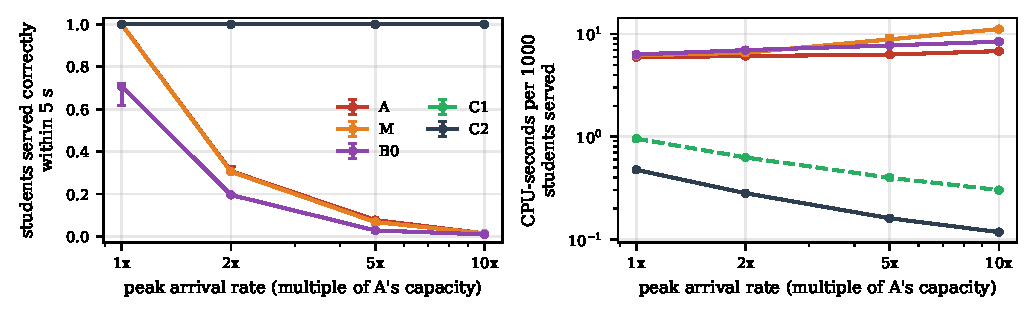
\includegraphics[width=\textwidth]{figures/core.pdf}
\caption{Q1. Left: share of students who got their correct result within
\SI{5}{s}. Right: CPU-seconds per \num{1000} students served (log scale).
Medians of 3 runs with 95\% bootstrap intervals; students do not refresh in
these runs. C1 (dashed) and C2 overlap at 100\%.}
\label{fig:core}
\end{figure*}

No run in any experiment returned a wrong result, and no container crashed.

\subsection{Q1: Which architecture?}
\label{sec:rq1}

Fig.~\ref{fig:core} compares five designs from 1$\times$ to 10$\times$ A's
capacity, with students who do not refresh so that every design faces the same
requests. A served every student within \SI{5}{s} at 1$\times$ but only
30.8\% at 2$\times$, 7.7\% at 5$\times$ and 1.4\% at 10$\times$; at
10$\times$ only 20.6\% got a result at all. Mirrors (M) matched A at 2$\times$
and did worse beyond it, using up to 1.64 times A's CPU per student. A cold
cache (B0) was worse than no cache, serving only 70.8\% within \SI{5}{s} even
at 1$\times$. The pre-computed designs C1 and C2 served every student at every
load, with 99th-percentile latencies below \SI{0.7}{ms}, and used 12.5 to 57.8
times less CPU per student than A. C1's capacity is at least \CapCOne\
students/s (33.6 times A's), where our generator ran out. Pre-computing all
\num{200000} results took 6.9--\SI{7.0}{s} (C1) and 9.4--\SI{9.8}{s} (C2).
With a page-building cost of \SI{2}{ms} or \SI{0}{ms} instead of \SI{5}{ms},
A and B0 served at least 99.8\% of students within \SI{5}{s} at the same load
as 2$\times$, so this assumption decides how much load a database-backed
portal can take. The cost order did not change: per student served, A used
2.6 (\SI{0}{ms}) to 9.7 (\SI{2}{ms}) times the CPU of C2, and B0 always used
more than A.

\subsection{Q2: Does a waiting room help?}
\label{sec:rq2}

\begin{table}[t]
\caption{Design A alone and behind a waiting room at 5$\times$ with refreshing students (median of 3 runs; run ends 135\,s after release).}
\label{tab:wr}
\centering
\footnotesize
\setlength{\tabcolsep}{2.5pt}
\begin{tabular}{@{}lrrrrr@{}}
\toprule
Waiting room & \multicolumn{2}{c}{Served (\%)} & Waiting & Wait & $\tau$ \\
\cmidrule(lr){2-3}
 & 10\,s & at all & at end (\%) & p50 (s) & \\
\midrule
none (A alone) & 6.1 & 43.3 & 0.0 & 0.2 & 0.09 \\
FIFO, token & 4.1 & 36.8 & 52.2 & 40.6 & 0.79 \\
FIFO, naive & 3.7 & 41.9 & 58.1 & 59.5 & 0.60 \\
lottery, token & 4.4 & 34.2 & 52.5 & 38.2 & 0.01 \\
lottery, naive & 3.8 & 41.8 & 58.1 & 59.8 & -0.01 \\
\bottomrule
\end{tabular}
\end{table}


Table~\ref{tab:wr} shows A alone and behind each waiting room at 5$\times$
with refreshing students. Within this \SI{135}{s} run the waiting room served
no more students than A alone (34.2--41.9\% against 43.3\%), but A's
unserved students had given up while 52--58\% of the waiting room's were
still queued. We therefore ran FIFO again with \SI{240}{s} more for the queue
to empty. It then served 98.3\% of students with naive tickets, but the
median student waited \SI{121}{s} to be admitted (95th percentile
\SI{282}{s}); in our model, queued students wait up to 10 minutes, and real
ones may leave sooner. With tokens it served only 74.5\%: admitted students
who ran out of patience refreshed straight at A, which received 3.21 requests
per student instead of 1.07. Only FIFO with tokens kept arrival order
(Kendall's $\tau=0.79$ between arrival and admission order for early
students, Table~\ref{tab:wr}); naive tickets lowered it to 0.60 because a
refresh sent the student to the back, and the lottery gave $\tau\approx0$,
like A alone. In front of C1, which needs no protection, the waiting room only added
delay and raised the CPU per \num{1000} students from 0.44 to 0.77--0.78
CPU-seconds.

\subsection{Q3: Are the results correct?}
\label{sec:rq3}

We published corrections for 1\% of students \SI{30}{s} after release at
1$\times$. Most students look once and had already looked, so corrected
students received only about 90 answers after the correction in the three
runs of each design. A, B0 with cache invalidation, and C1 gave at most one
old result, while the correction was being written (it finished within
\SI{0.19}{s}). B0 without invalidation served old results for up to
\SI{10.89}{s}, and would until its 10-minute lifetime ended; C2 served old
files from Nginx's 30-second file cache for up to \SI{13.69}{s}. When only
90\% of results were ready at release, C1 wrote the rest in \SI{0.08}{s} and
C2 in \SI{1.63}{s}, and one student was told ``not found''; a slower
preparation would leave more students without a result for longer.

\subsection{Q4: Caches and refreshing students}
\label{sec:rq4}

At 2$\times$, with every student asking for a different roll number, every
cache miss in B0 was the first request for that key; no two requests ever
raced for the same key. Request coalescing (B1) and early recomputation (B2)
therefore changed nothing (8.5--8.9\% served within \SI{5}{s}), while filling
the cache before release (B3) served everyone, at 0.71 CPU-seconds per
\num{1000} students against B0's 6.27.

\begin{figure*}[t]
\centering
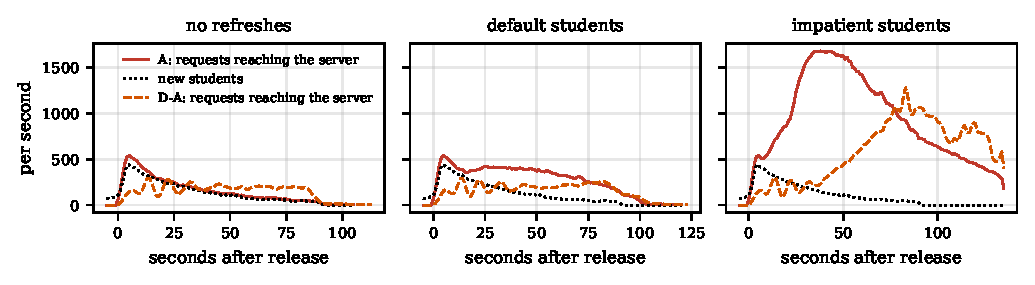
\includegraphics[width=\textwidth]{figures/refresh.pdf}
\caption{Q4. Requests reaching the server each second for A alone (solid) and
behind a waiting room (D-A, dashed) at 2$\times$, against new students
(dotted). One run per kind of student.}
\label{fig:refresh}
\end{figure*}

Refreshing changes the load a lot (Fig.~\ref{fig:refresh}). For A at
2$\times$, students who never
refresh sent 1.17 requests each; our default students sent 2.23, so more were
served in the end (88.1\% against 77.7\%) but fewer within \SI{10}{s} (32.7\%
against 53.7\%). Impatient students (patience 3--\SI{8}{s}) sent 8.65 requests
each and kept A overloaded until the end of every run; only 22.1\% were
served. Behind a waiting room the load on A stayed near one request per
student with default students (1.32), but with impatient students A still
received 5.30 requests per student.

\subsection{Decision guide}

\begin{table}[t]
\caption{Decision guide for examination boards, from our measurements}
\label{tab:guide}
\centering
\footnotesize
\setlength{\tabcolsep}{3pt}
\begin{tabular}{@{}>{\raggedright\arraybackslash}p{2.5cm}>{\raggedright\arraybackslash}p{3.1cm}>{\raggedright\arraybackslash}p{2.3cm}@{}}
\toprule
If the board\ldots & then\ldots & because (section)\\
\midrule
has the results before release & publishes them pre-computed, as files or in a key--value store & served 10$\times$ at 12.5--57.8$\times$ less CPU (\ref{sec:rq1})\\
must build pages from a database & does not count on mirrors or an empty cache; fills the cache before release & M and B0 no better than A; B3 served all (\ref{sec:rq1}, \ref{sec:rq4})\\
cannot finish preparing by release time & delays the release & early students are told ``not found'' (\ref{sec:rq3})\\
corrects results after release & deletes or rewrites every cached copy and keeps file caches short & old results for up to \SI{14}{s} otherwise (\ref{sec:rq3})\\
expects students to refresh & makes the page retry by itself, with back-off & impatient students kept A down (\ref{sec:rq4})\\
considers a waiting room in front of a slow website & uses one only if students can wait minutes; admits FIFO; does not let admitted students refresh without limit & served 98.3\% instead of 43.3\%, after a \SI{121}{s} median wait; 74.5\% with tokens (\ref{sec:rq2})\\
\bottomrule
\end{tabular}
\end{table}

Table~\ref{tab:guide} turns these results into advice. The numbers come from
one machine and should be read as relative, not absolute.

\textbf{Limitations.} All runs used one machine, no content delivery network
and a surge compressed to \SI{90}{s}. The students and the page-building cost
are models. Three runs per configuration give wide intervals for some
measures. We have not yet measured a real result day.
